\documentclass[tikz,border=8pt]{standalone}
\usepackage{amsmath}
\usetikzlibrary{arrows.meta,positioning,fit,calc}

\begin{document}
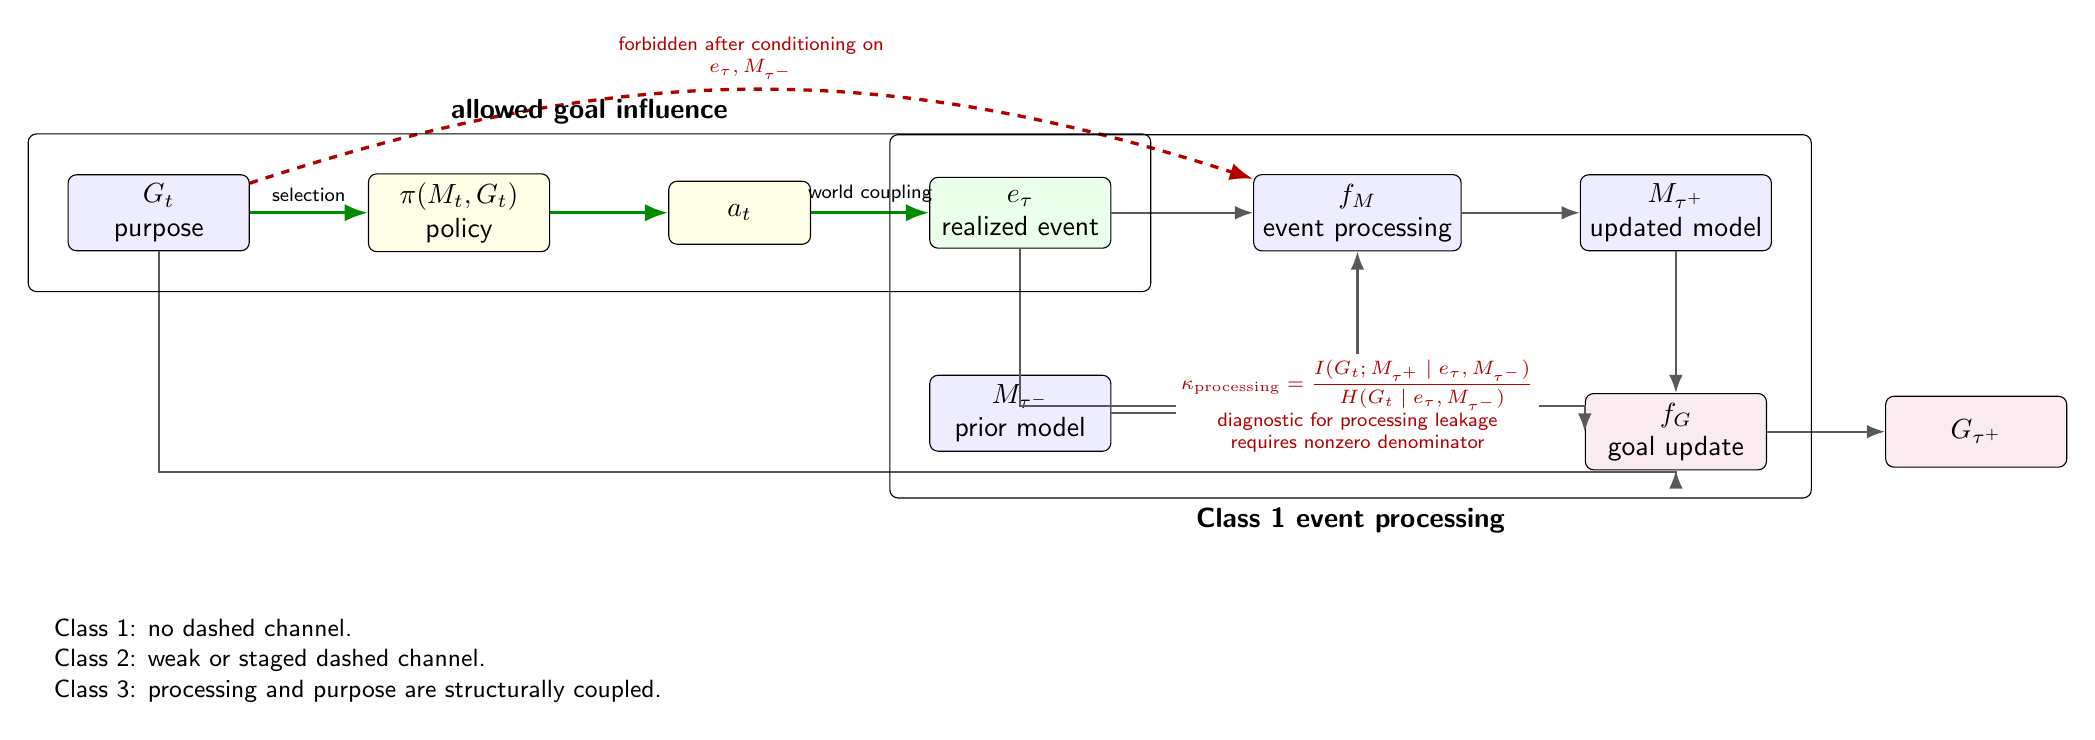
\begin{tikzpicture}[
  font=\sffamily,
  node distance=10mm and 15mm,
  box/.style={draw, rounded corners=3pt, align=center, minimum width=23mm, minimum height=9mm, fill=white},
  smallbox/.style={draw, rounded corners=3pt, align=center, minimum width=18mm, minimum height=8mm, fill=white},
  allowed/.style={-Latex, very thick, draw=green!55!black},
  neutral/.style={-Latex, thick, draw=black!65},
  forbidden/.style={-Latex, very thick, draw=red!70!black, dashed},
  note/.style={align=center, font=\sffamily\scriptsize},
  title/.style={font=\sffamily\bfseries}
]

\node[box, fill=blue!7] (g) {$G_t$\\purpose};
\node[box, right=of g, fill=yellow!10] (pi) {$\pi(M_t,G_t)$\\policy};
\node[smallbox, right=of pi, fill=yellow!10] (a) {$a_t$};
\node[box, right=of a, fill=green!8] (e) {$e_\tau$\\realized event};
\node[box, below=16mm of e, fill=blue!7] (m0) {$M_{\tau^-}$\\prior model};
\node[box, right=18mm of e, fill=blue!7] (fm) {$f_M$\\event processing};
\node[box, right=of fm, fill=blue!7] (m1) {$M_{\tau^+}$\\updated model};
\node[box, below=18mm of m1, fill=purple!8] (fg) {$f_G$\\goal update};
\node[box, right=of fg, fill=purple!8] (g1) {$G_{\tau^+}$};

\draw[allowed] (g) -- node[above, note] {selection} (pi);
\draw[allowed] (pi) -- (a);
\draw[allowed] (a) -- node[above, note] {world coupling} (e);
\draw[neutral] (e) -- (fm);
\draw[neutral] (m0) -| (fm);
\draw[neutral] (fm) -- (m1);
\draw[neutral] (m1) -- (fg);
\draw[neutral] (g.south) -- ++(0,-28mm) -| (fg.south);
\draw[neutral] (e.south) -- ++(0,-20mm) -| (fg.west);
\draw[neutral] (fg) -- (g1);

\draw[forbidden] (g) to[bend left=18] node[above, note, text=red!70!black] {forbidden after conditioning on\\$e_\tau,M_{\tau^-}$} (fm);

\node[note, below=13mm of fm, text=red!70!black, fill=white, inner sep=2pt] (kappa)
  {$\displaystyle \kappa_{\mathrm{processing}}=
  \frac{I(G_t;M_{\tau^+}\mid e_\tau,M_{\tau^-})}
       {H(G_t\mid e_\tau,M_{\tau^-})}$\\
  diagnostic for processing leakage\\
  requires nonzero denominator};

\node[draw, rounded corners=3pt, fit=(g)(pi)(a)(e), inner sep=5mm, label={[title]above:allowed goal influence}] {};
\node[draw, rounded corners=3pt, fit=(m0)(fm)(m1)(kappa), inner sep=5mm, label={[title]below:Class 1 event processing}] {};

\node[anchor=west, align=left, font=\sffamily\small] at ($(g.south west)+(-3mm,-52mm)$) {
Class 1: no dashed channel.\\
Class 2: weak or staged dashed channel.\\
Class 3: processing and purpose are structurally coupled.
};

\end{tikzpicture}
\end{document}
